\documentclass{article}

\usepackage{csc579}
\usepackage{amssymb,amsmath,amsthm}
\usepackage{tikz}
\usepackage{multicol}
\usepackage{enumitem}
\usepackage{gensymb}
\usepackage[T1]{fontenc}
\usepackage{inconsolata}
\usepackage{qtree}
\usepackage{pgfplots}
\usepackage{hyperref}
\pgfplotsset{compat=1.7}

\thickmuskip=2mu

\begin{document}

\HWK{Project 2}{March 27, 2017}

\bigskip

\textbf{Task 1 (M/M/1/K System)}
Let $\mu = 1$ as before, the size of the queue $K = 40$, and the number of customers served before a simulation run terminates $C = 100,000$. Plot the average customer waiting time against the value of $\rho$, for $\rho = 0.05$ to $\rho = 0.95$, in increments of 0.10 (remember to include the confidence intervals). Compile five plots, one for each of the service disciplines. In particular, for the Priority service disciplines, plot the average waiting time of each of the four classes of customers, as well as the overall average. Compare and discuss the results, and submit these graphs along with your code.
\\
\medskip\\\texttt{
\\
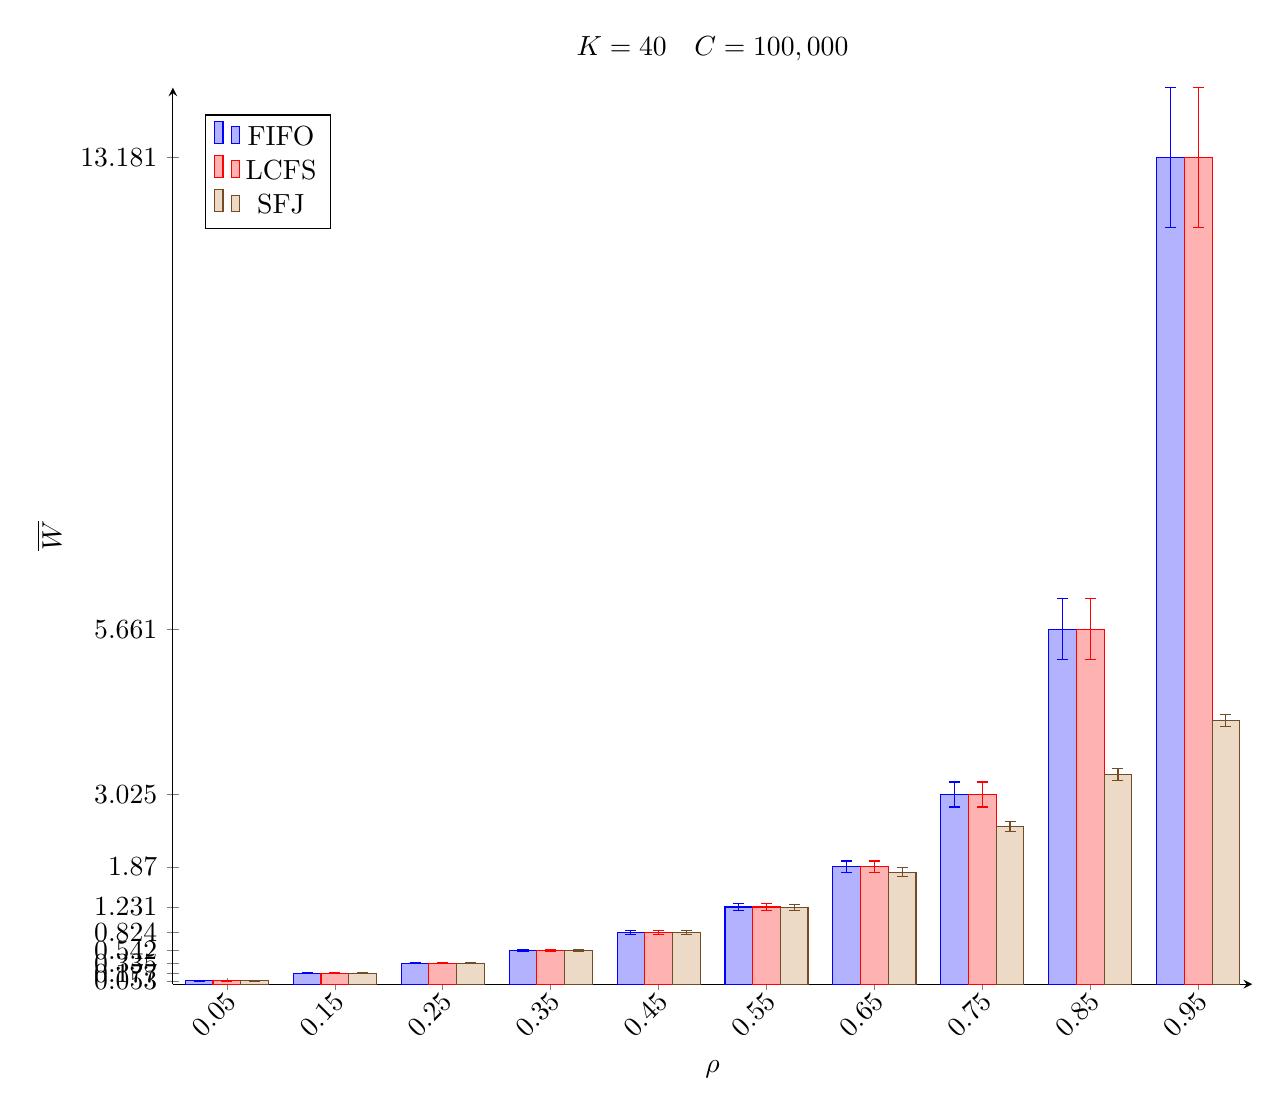
\begin{tikzpicture}[scale=1.0]
\begin{axis}[
    legend pos=north west,
    title= {$K=40 \quad C=100,000$},  
	ymin=0,
	y post scale=2,
	x post scale=2,
	ybar=0pt,
	enlargelimits={abs=0.5},
    xmin=0,
    xmax=1,
	xlabel = {$\rho$},
    ylabel = {$\overline{W}$},
	xtick=data,
	ytick=data,
	ticklabel style={
        /pgf/number format/fixed,
        /pgf/number format/precision=5
	},
	x tick label style={rotate=45, anchor=east, align=center, xshift=.1cm,yshift=-0.1cm},
	axis lines=left
	]
\addplot+[error bars/.cd,
y dir=both,y explicit]
coordinates {
    (.05,0.053) +- (0.0, 0.003)
    (.15,0.177) +- (0.0, 0.006)
    (.25,0.335) +- (0.0, 0.010)
    (.35,0.542) +- (0.0, 0.017)
    (.45,0.824) +- (0.0, 0.030)
    (.55,1.231) +- (0.0, 0.052)
    (.65,1.870) +- (0.0, 0.094)
    (.75,3.025) +- (0.0, 0.199)
    (.85,5.661) +- (0.0, 0.487)
    (.95,13.181) +- (0.0, 1.117)};
\addplot+[error bars/.cd,
y dir=both,y explicit]
coordinates {
    (.05,0.053) +- (0.0, 0.003)
    (.15,0.177) +- (0.0, 0.006)
    (.25,0.335) +- (0.0, 0.010)
    (.35,0.542) +- (0.0, 0.017)
    (.45,0.824) +- (0.0, 0.030)
    (.55,1.231) +- (0.0, 0.052)
    (.65,1.870) +- (0.0, 0.094)
    (.75,3.025) +- (0.0, 0.199)
    (.85,5.661) +- (0.0, 0.487)
    (.95,13.181) +- (0.0, 1.117)};
\addplot+[error bars/.cd,
y dir=both,y explicit]
coordinates {
    (.05,0.053) +- (0.0, 0.003)
    (.15,0.177) +- (0.0, 0.006)
    (.25,0.335) +- (0.0, 0.010)
    (.35,0.542) +- (0.0, 0.017)
    (.45,0.824) +- (0.0, 0.030)
    (.55,1.223) +- (0.0, 0.050)
    (.65,1.786) +- (0.0, 0.069)
    (.75,2.516) +- (0.0, 0.081)
    (.85,3.348) +- (0.0, 0.098)
    (.95,4.202) +- (0.0, 0.095)};
\legend{FIFO, LCFS, SFJ}
\end{axis}
\end{tikzpicture}
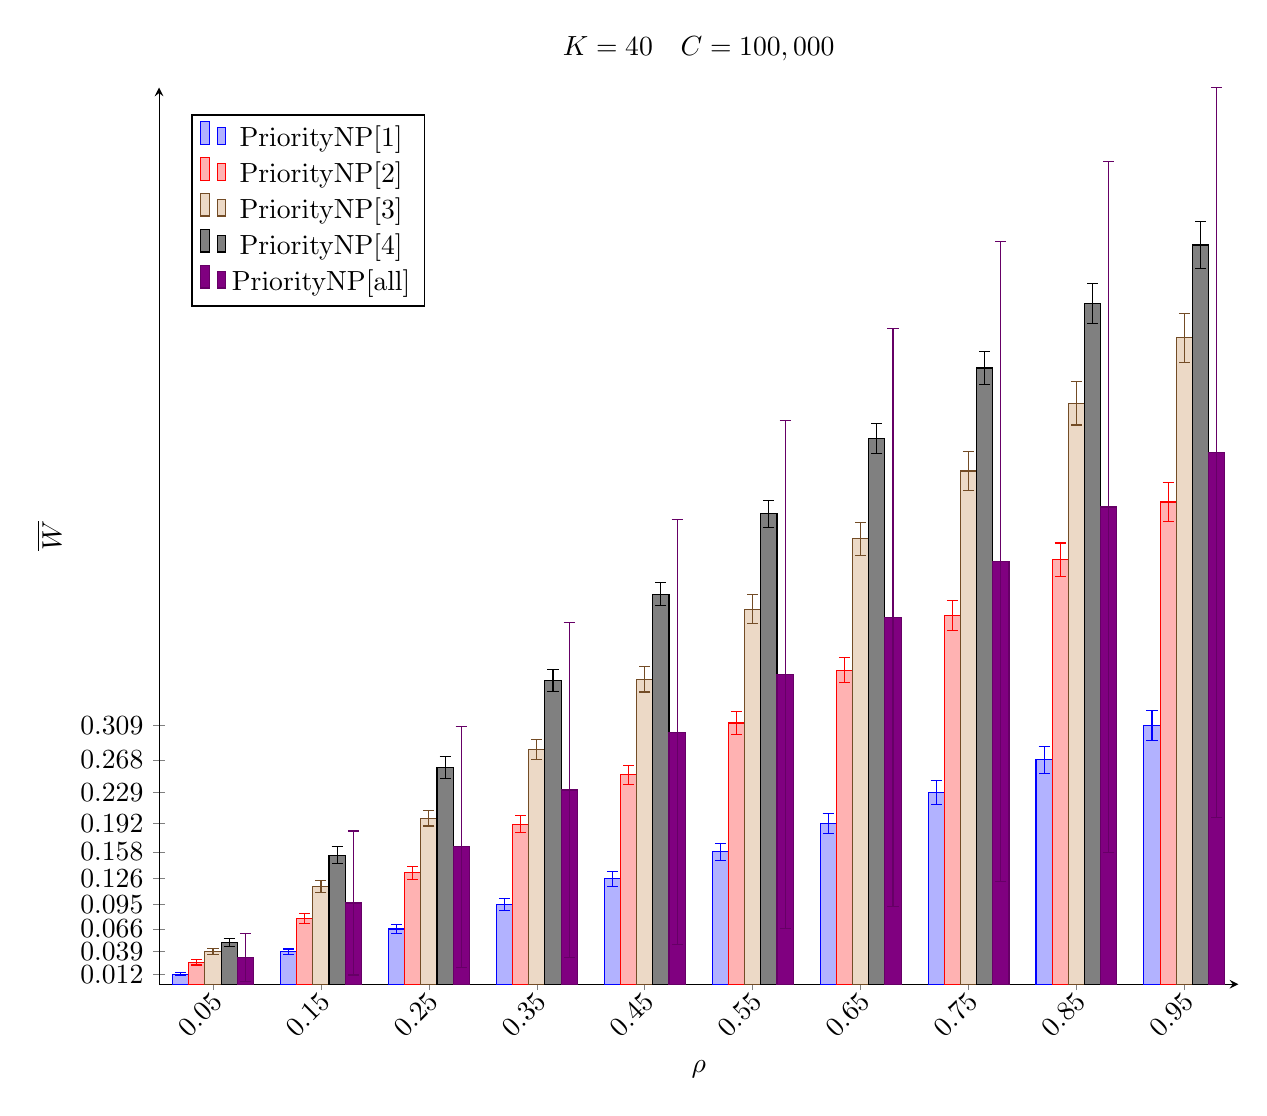
\begin{tikzpicture}
\begin{axis}[
    legend pos=north west,
    title= {$K=40 \quad C=100,000$},  
	ymin=0,
	y post scale=2,
	x post scale=2,
	ybar=0pt,
	bar width=0.015,
	enlargelimits={abs=0.5},
    xmin=0,
    xmax=1,
	xlabel = {$\rho$},
    ylabel = {$\overline{W}$},
	xtick=data,
	ytick=data,
	ticklabel style={
        /pgf/number format/fixed,
        /pgf/number format/precision=5
	},
	x tick label style={rotate=45, anchor=east, align=center, xshift=.1cm,yshift=-0.1cm},
	axis lines=left
	]
\addplot+[error bars/.cd,
y dir=both,y explicit]
coordinates {
    (.05,0.012) +- (0.0,0.002)
    (.15,0.039) +- (0.0,0.003)
    (.25,0.066) +- (0.0,0.005)
    (.35,0.095) +- (0.0,0.007)
    (.45,0.126) +- (0.0,0.009)
    (.55,0.158) +- (0.0,0.010)
    (.65,0.192) +- (0.0,0.012)
    (.75,0.229) +- (0.0,0.014)
    (.85,0.268) +- (0.0,0.016)
    (.95,0.309) +- (0.0,0.018)
};
\addplot+[error bars/.cd,
y dir=both,y explicit]
coordinates {
    (.05,0.026) +- (0.0,0.003)
    (.15,0.078) +- (0.0,0.006)
    (.25,0.133) +- (0.0,0.008)
    (.35,0.191) +- (0.0,0.010)
    (.45,0.250) +- (0.0,0.011)
    (.55,0.312) +- (0.0,0.014)
    (.65,0.375) +- (0.0,0.015)
    (.75,0.440) +- (0.0,0.018)
    (.85,0.507) +- (0.0,0.020)
    (.95,0.576) +- (0.0,0.023)
};
\addplot+[error bars/.cd,
y dir=both,y explicit]
coordinates {
    (.05,0.039) +- (0.0,0.004)
    (.15,0.117) +- (0.0,0.007)
    (.25,0.198) +- (0.0,0.009)
    (.35,0.280) +- (0.0,0.012)
    (.45,0.364) +- (0.0,0.015)
    (.55,0.448) +- (0.0,0.017)
    (.65,0.532) +- (0.0,0.020)
    (.75,0.613) +- (0.0,0.023)
    (.85,0.694) +- (0.0,0.026)
    (.95,0.772) +- (0.0,0.029)
};
\addplot+[error bars/.cd,
y dir=both,y explicit]
coordinates {
    (.05,0.050) +- (0.0,0.005)
    (.15,0.154) +- (0.0,0.010)
    (.25,0.259) +- (0.0,0.013)
    (.35,0.363) +- (0.0,0.013)
    (.45,0.466) +- (0.0,0.014)
    (.55,0.562) +- (0.0,0.016)
    (.65,0.652) +- (0.0,0.018)
    (.75,0.736) +- (0.0,0.020)
    (.85,0.813) +- (0.0,0.024)
    (.95,0.883) +- (0.0,0.028)
};
\addplot+[error bars/.cd,
y dir=both,y explicit]
coordinates {
    (.05,0.032) +- (0.0,0.029)
    (.15,0.097) +- (0.0, 0.086)
    (.25,0.164) +- (0.0, 0.144)
    (.35,0.232) +- (0.0, 0.200)
    (.45,0.301) +- (0.0, 0.254)
    (.55,0.370) +- (0.0, 0.303)
    (.65,0.438) +- (0.0, 0.345)
    (.75,0.505) +- (0.0, 0.382)
    (.85,0.570) +- (0.0, 0.413)
    (.95,0.635) +- (0.0, 0.436)
};
\legend{PriorityNP[1], PriorityNP[2], PriorityNP[3], PriorityNP[4], PriorityNP[all]}
\end{axis}
\end{tikzpicture}
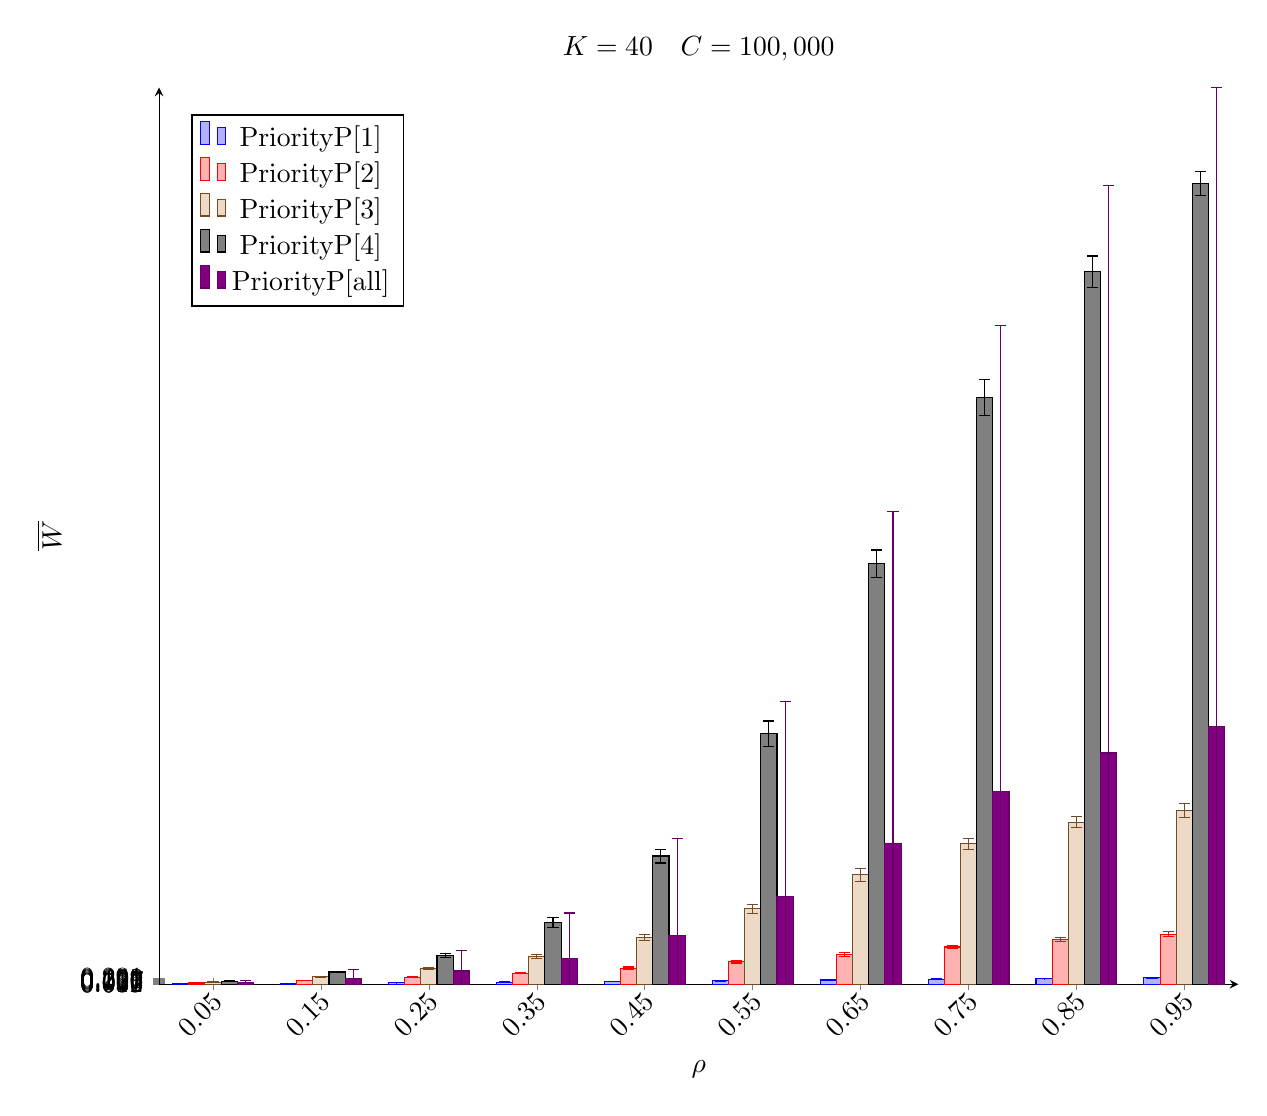
\begin{tikzpicture}
\begin{axis}[
    legend pos=north west,
    title= {$K=40 \quad C=100,000$},  
	ymin=0,
	y post scale=2,
	x post scale=2,
	ybar=0pt,
	bar width=0.015,
	enlargelimits={abs=0.5},
    xmin=0,
    xmax=1,
	xlabel = {$\rho$},
    ylabel = {$\overline{W}$},
	xtick=data,
	ytick=data,
	ticklabel style={
        /pgf/number format/fixed,
        /pgf/number format/precision=5
	},
	x tick label style={rotate=45, anchor=east, align=center, xshift=.1cm,yshift=-0.1cm},
	axis lines=left
	]
\addplot+[error bars/.cd,
y dir=both,y explicit]
coordinates {
    (.05,0.012) +- (0.0,0.002)
    (.15,0.039) +- (0.0,0.003)
    (.25,0.066) +- (0.0,0.005)
    (.35,0.095) +- (0.0,0.006)
    (.45,0.127) +- (0.0,0.008)
    (.55,0.157) +- (0.0,0.010)
    (.65,0.191) +- (0.0,0.011)
    (.75,0.226) +- (0.0,0.013)
    (.85,0.259) +- (0.0,0.011)
    (.95,0.291) +- (0.0,0.014)
};
\addplot+[error bars/.cd,
y dir=both,y explicit]
coordinates {
    (.05,0.053) +- (0.0,0.005)
    (.15,0.175) +- (0.0,0.009)
    (.25,0.321) +- (0.0,0.017)
    (.35,0.507) +- (0.0,0.028)
    (.45,0.735) +- (0.0,0.051)
    (.55,1.028) +- (0.0,0.061) 
    (.65,1.370) +- (0.0,0.088)
    (.75,1.697) +- (0.0,0.077)
    (.85,2.032) +- (0.0,0.098) 
    (.95,2.281) +- (0.0,0.105)
};
\addplot+[error bars/.cd,
y dir=both,y explicit]
coordinates {
    (.05,0.096) +- (0.0,0.008)
    (.15,0.342) +- (0.0,0.016)
    (.25,0.703) +- (0.0,0.045)
    (.35,1.258) +- (0.0,0.080)
    (.45,2.132) +- (0.0,0.143) 
    (.55,3.438) +- (0.0,0.210) 
    (.65,4.988) +- (0.0,0.290)
    (.75,6.397) +- (0.0,0.242)
    (.85,7.387) +- (0.0,0.249)
    (.95,7.927) +- (0.0,0.319)
};
\addplot+[error bars/.cd,
y dir=both,y explicit]
coordinates {
    (.05,0.141) +- (0.0,0.008)
    (.15,0.558) +- (0.0,0.025)
    (.25,1.313) +- (0.0,0.091)
    (.35,2.810) +- (0.0,0.239)
    (.45,5.840) +- (0.0,0.317)
    (.55,11.411) +- (0.0,0.585)
    (.65,19.162) +- (0.0,0.628)
    (.75,26.741) +- (0.0,0.806)
    (.85,32.469) +- (0.0,0.717)
    (.95,36.488) +- (0.0,0.536)
};
\addplot+[error bars/.cd,
y dir=both,y explicit]
coordinates {
    (.05,0.075) +- (0.0,0.096)
    (.15,0.278) +- (0.0, 0.388)
    (.25,0.601) +- (0.0, 0.941)
    (.35,1.168) +- (0.0, 2.076)
    (.45,2.208) +- (0.0, 4.442)
    (.55,4.009) +- (0.0, 8.885)
    (.65,6.428) +- (0.0, 15.127)
    (.75,8.765) +- (0.0, 21.256)
    (.85,10.537) +- (0.0, 25.866)
    (.95,11.747) +- (0.0, 29.115)
};
\legend{PriorityP[1], PriorityP[2], PriorityP[3], PriorityP[4], PriorityP[all]}
\end{axis}
\end{tikzpicture}
\\
For a constant queue capacity and completion size, where the queue capacity is large relative to the average number of customers in the system, the $\overline{W}$  increases quickly at higher values of $\rho$. The FIFO and LCFS scheduling policies yield exactly the same average wait times, since there are only two components to calculating average wait time: the residual customers currently in service (because non-preemptive), and the waiting time due to jobs that arrive after the a specific job arrives, but before it enters service. These do not change between FIFO and LCFS.\\
SJF shows a lower overal wait time.\\
The preemptive priority queue has a slightly reduced $\overline{W}$ for queue1 compared to the non-preemptive implementation at higher values of $\rho$, but at the high cost of much longer wait times for the other queues.
}
\bigskip
\newpage


%%%%%%%%%%%%%%%%%%%%%%
%%%%%%%%%%%%%%%%%%%%%%
%%%%%%%%%%%%%%%%%%%%%%

\textbf{Task 2 (M/M/1/K System)}
Let $K = 20$ and $C = 100,000$. Compute and plot the CLR for $\rho = 0.05, · · · , 0.95$, in increments of 0.10. Also determine and plot the running time of your simulation for the same values of $\rho$ (use $C = 1, 000, 000$ customers). Produce five plots as in Task 1 for each performance metric (CLR and running time);
also compute confidence intervals. How does the behavior of the plots change as a function of (i) the service discipline, and (ii) preemption/non-preemption, for the Priority disciplines? Can you explain this behavior?
\\
\medskip\\\texttt{
\\
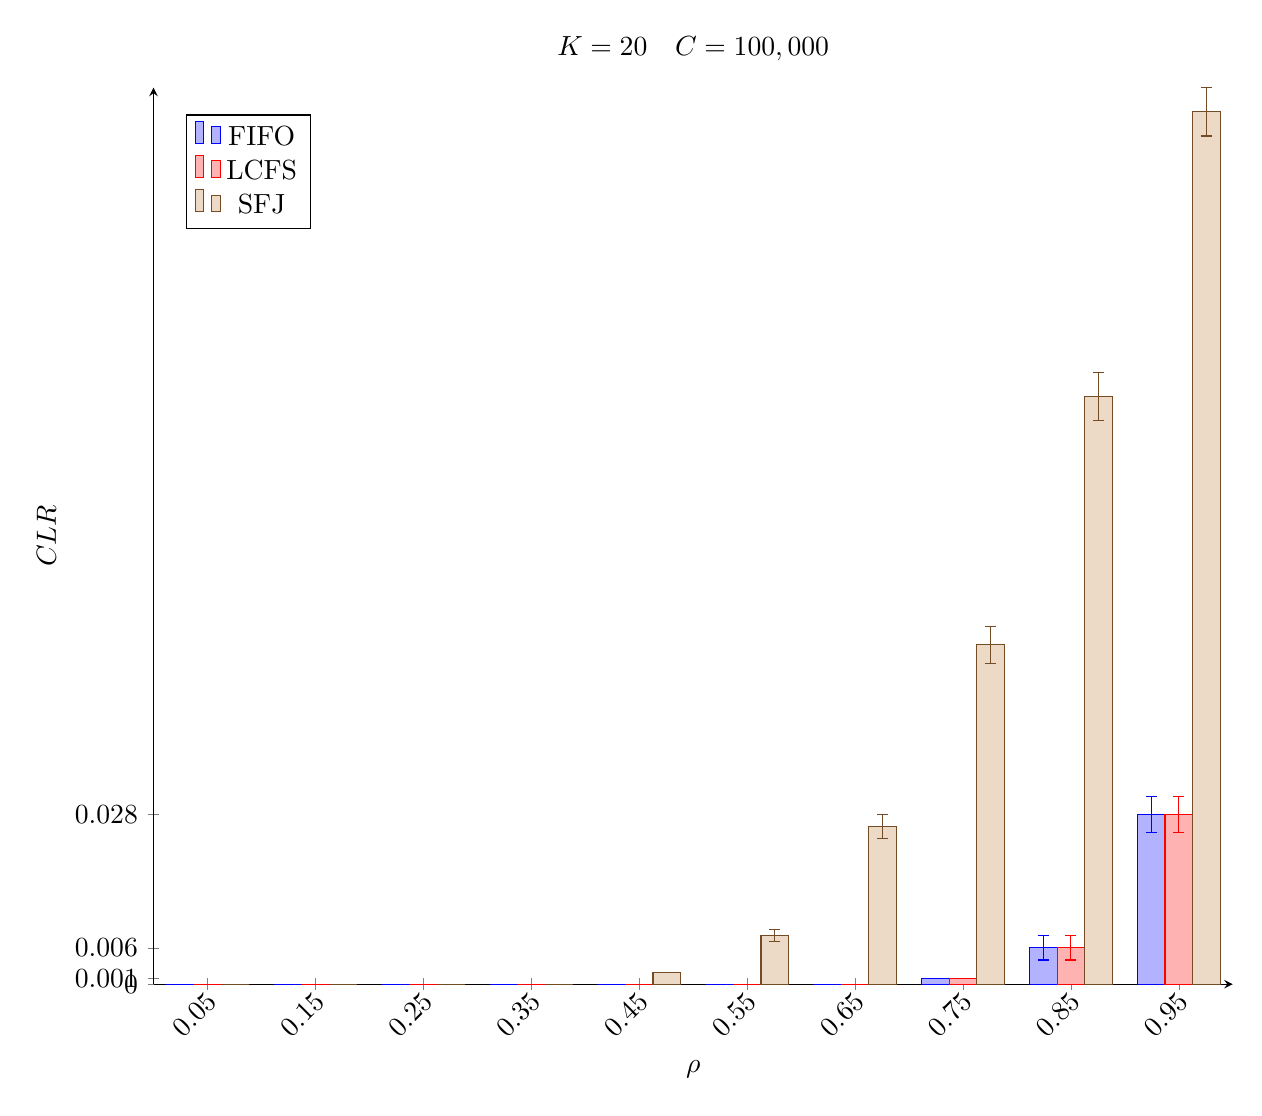
\begin{tikzpicture}[scale=1.0]
\begin{axis}[
    legend pos=north west,
    title= {$K=20 \quad C=100,000$},  
	ymin=0,
	y post scale=2,
	x post scale=2,
	ybar=0pt,
	enlargelimits={abs=0.5},
    xmin=0,
    xmax=1,
	xlabel = {$\rho$},
    ylabel = {$CLR$},
	xtick=data,
	ytick=data,
	ticklabel style={
        /pgf/number format/fixed,
        /pgf/number format/precision=5
	},
	x tick label style={rotate=45, anchor=east, align=center, xshift=.1cm,yshift=-0.1cm},
	axis lines=left
	]
\addplot+[error bars/.cd,
y dir=both,y explicit]
coordinates {
    (0.05,0.000) +- (0.0,0.000)
    (0.15,0.000) +- (0.0,0.000)
    (0.25,0.000) +- (0.0,0.000)
    (0.35,0.000) +- (0.0,0.000)
    (0.45,0.000) +- (0.0,0.000)
    (0.55,0.000) +- (0.0,0.000)
    (0.65,0.000) +- (0.0,0.000)
    (0.75,0.001) +- (0.0,0.000)
    (0.85,0.006) +- (0.0,0.002)
    (0.95,0.028) +- (0.0,0.003)
};
\addplot+[error bars/.cd,
y dir=both,y explicit]
coordinates {
    (0.05,0.000) +- (0.0,0.000)
    (0.15,0.000) +- (0.0,0.000)
    (0.25,0.000) +- (0.0,0.000)
    (0.35,0.000) +- (0.0,0.000)
    (0.45,0.000) +- (0.0,0.000)
    (0.55,0.000) +- (0.0,0.000)
    (0.65,0.000) +- (0.0,0.000)
    (0.75,0.001) +- (0.0,0.000)
    (0.85,0.006) +- (0.0,0.002)
    (0.95,0.028) +- (0.0,0.003)
};
\addplot+[error bars/.cd,
y dir=both,y explicit]
coordinates {
    (0.05,0.000) +- (0.0,0.000)
    (0.15,0.000) +- (0.0,0.000)
    (0.25,0.000) +- (0.0,0.000)
    (0.35,0.000) +- (0.0,0.000)
    (0.45,0.002) +- (0.0,0.000)
    (0.55,0.008) +- (0.0,0.001)
    (0.65,0.026) +- (0.0,0.002)
    (0.75,0.056) +- (0.0,0.003)
    (0.85,0.097) +- (0.0,0.004)
    (0.95,0.144) +- (0.0,0.004)
};
\legend{FIFO, LCFS, SFJ}
\end{axis}
\end{tikzpicture}
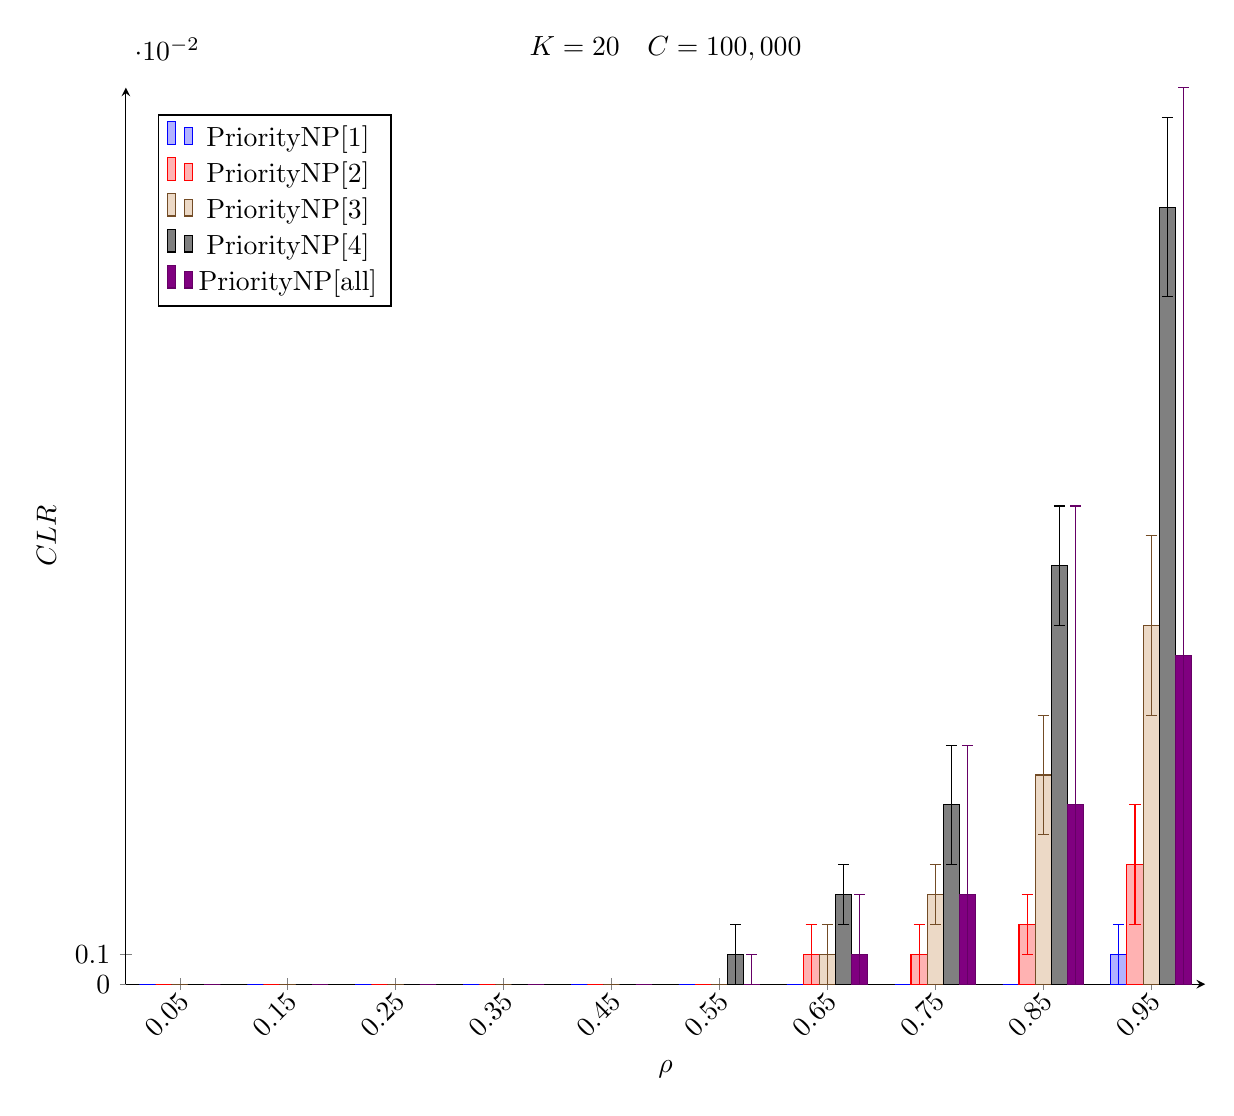
\begin{tikzpicture}
\begin{axis}[
    legend pos=north west,
    title= {$K=20 \quad C=100,000$},  
	ymin=0,
	y post scale=2,
	x post scale=2,
	ybar=0pt,
	bar width=0.015,
	enlargelimits={abs=0.5},
    xmin=0,
    xmax=1,
	xlabel = {$\rho$},
    ylabel = {$CLR$},
	xtick=data,
	ytick=data,
	ticklabel style={
        /pgf/number format/fixed,
        /pgf/number format/precision=5
	},
	x tick label style={rotate=45, anchor=east, align=center, xshift=.1cm,yshift=-0.1cm},
	axis lines=left
	]
\addplot+[error bars/.cd,
y dir=both,y explicit]
coordinates {
    (0.05,0.000) +- (0.0,0.000)
    (0.15,0.000) +- (0.0,0.000)
    (0.25,0.000) +- (0.0,0.000)
    (0.35,0.000) +- (0.0,0.000)
    (0.45,0.000) +- (0.0,0.000)
    (0.55,0.000) +- (0.0,0.000)
    (0.65,0.000) +- (0.0,0.000)
    (0.75,0.000) +- (0.0,0.000)
    (0.85,0.000) +- (0.0,0.000)
    (0.95,0.001) +- (0.0,0.001)
};
\addplot+[error bars/.cd,
y dir=both,y explicit]
coordinates {
    (0.05,0.000) +- (0.0,0.000)
    (0.15,0.000) +- (0.0,0.000)
    (0.25,0.000) +- (0.0,0.000)
    (0.35,0.000) +- (0.0,0.000)
    (0.45,0.000) +- (0.0,0.000)
    (0.55,0.000) +- (0.0,0.000)
    (0.65,0.001) +- (0.0,0.001)
    (0.75,0.001) +- (0.0,0.001)
    (0.85,0.002) +- (0.0,0.001)
    (0.95,0.004) +- (0.0,0.002)
};
\addplot+[error bars/.cd,
y dir=both,y explicit]
coordinates {
    (0.05,0.000) +- (0.0,0.000)
    (0.15,0.000) +- (0.0,0.000)
    (0.25,0.000) +- (0.0,0.000)
    (0.35,0.000) +- (0.0,0.000)
    (0.45,0.000) +- (0.0,0.000)
    (0.55,0.000) +- (0.0,0.000)
    (0.65,0.001) +- (0.0,0.001)
    (0.75,0.003) +- (0.0,0.001)
    (0.85,0.007) +- (0.0,0.002)
    (0.95,0.012) +- (0.0,0.003)
};
\addplot+[error bars/.cd,
y dir=both,y explicit]
coordinates {
    (0.05,0.000) +- (0.0,0.000)
    (0.15,0.000) +- (0.0,0.000)
    (0.25,0.000) +- (0.0,0.000)
    (0.35,0.000) +- (0.0,0.000)
    (0.45,0.000) +- (0.0,0.000)
    (0.55,0.001) +- (0.0,0.001)
    (0.65,0.003) +- (0.0,0.001)
    (0.75,0.006) +- (0.0,0.002)
    (0.85,0.014) +- (0.0,0.002)
    (0.95,0.026) +- (0.0,0.003)
};
\addplot+[error bars/.cd,
y dir=both,y explicit]
coordinates {
    (0.05,0.000) +- (0.0,0.000)
    (0.15,0.000) +- (0.0,0.000)
    (0.25,0.000) +- (0.0,0.000)
    (0.35,0.000) +- (0.0,0.000)
    (0.45,0.000) +- (0.0,0.000)
    (0.55,0.000) +- (0.0,0.001)
    (0.65,0.001) +- (0.0,0.002)
    (0.75,0.003) +- (0.0,0.005)
    (0.85,0.006) +- (0.0,0.010)
    (0.95,0.011) +- (0.0,0.019)
};
\legend{PriorityNP[1], PriorityNP[2], PriorityNP[3], PriorityNP[4], PriorityNP[all]}
\end{axis}
\end{tikzpicture}
\\
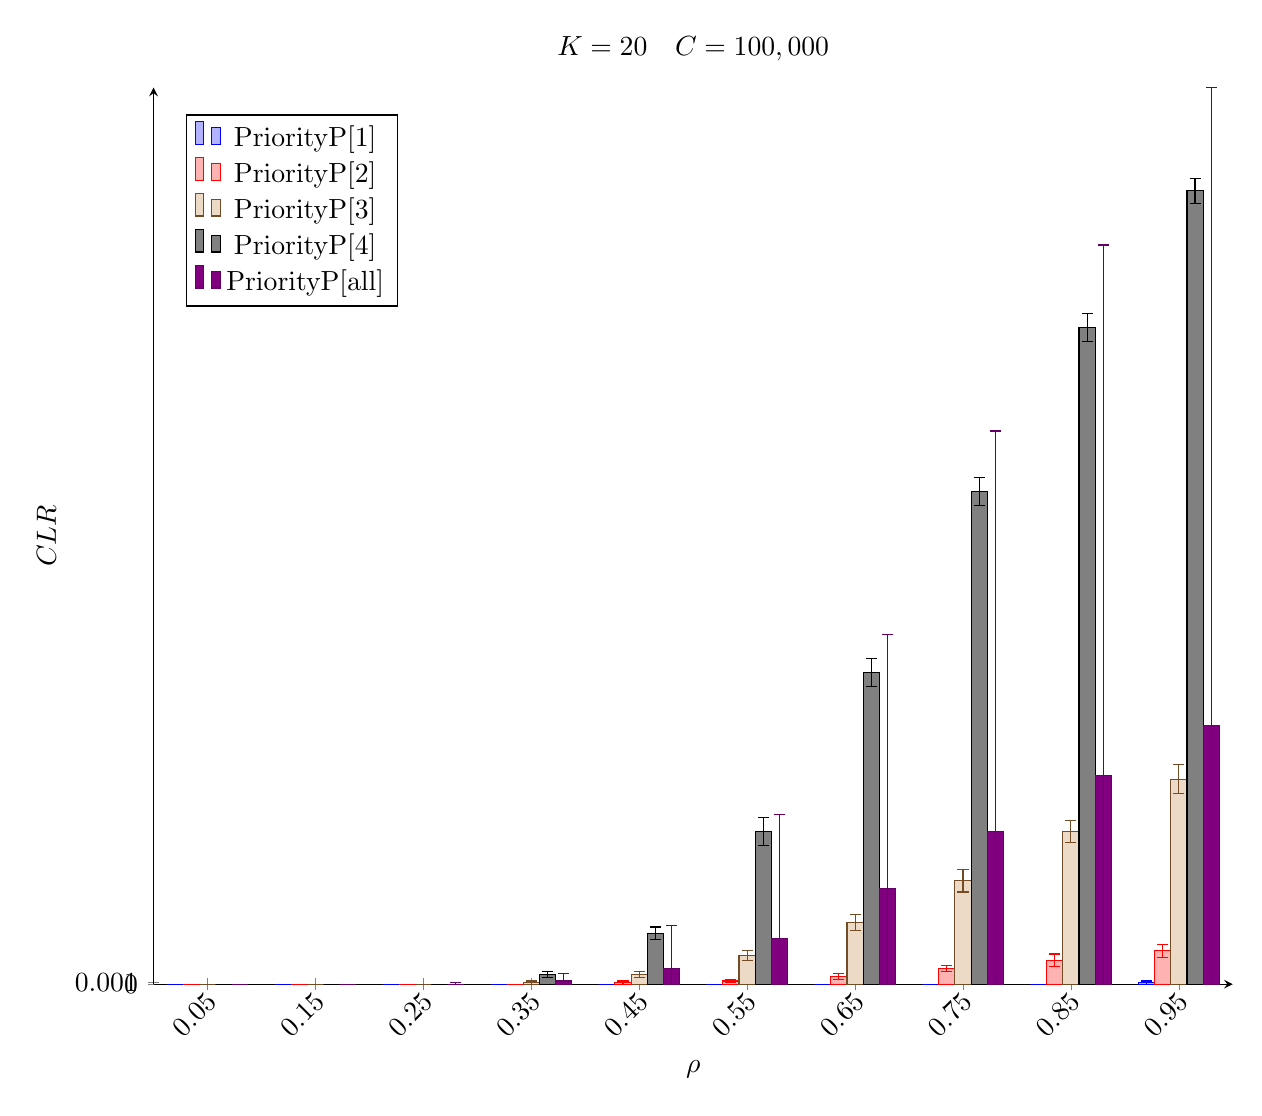
\begin{tikzpicture}
\begin{axis}[
    legend pos=north west,
    title= {$K=20 \quad C=100,000$},  
	ymin=0,
	y post scale=2,
	x post scale=2,
	ybar=0pt,
	bar width=0.015,
	enlargelimits={abs=0.5},
    xmin=0,
    xmax=1,
	xlabel = {$\rho$},
    ylabel = {$CLR$},
	xtick=data,
	ytick=data,
	ticklabel style={
        /pgf/number format/fixed,
        /pgf/number format/precision=5
	},
	x tick label style={rotate=45, anchor=east, align=center, xshift=.1cm,yshift=-0.1cm},
	axis lines=left
	]
\addplot+[error bars/.cd,
y dir=both,y explicit]
coordinates {
    (0.05,0.000) +- (0.0,0.000)
    (0.15,0.000) +- (0.0,0.000)
    (0.25,0.000) +- (0.0,0.000)
    (0.35,0.000) +- (0.0,0.000)
    (0.45,0.000) +- (0.0,0.000)
    (0.55,0.000) +- (0.0,0.000)
    (0.65,0.000) +- (0.0,0.000)
    (0.75,0.000) +- (0.0,0.000)
    (0.85,0.000) +- (0.0,0.000)
    (0.95,0.001) +- (0.0,0.001)
};
\addplot+[error bars/.cd,
y dir=both,y explicit]
coordinates {
    (0.05,0.000) +- (0.0,0.000)
    (0.15,0.000) +- (0.0,0.000)
    (0.25,0.000) +- (0.0,0.000)
    (0.35,0.000) +- (0.0,0.000)
    (0.45,0.001) +- (0.0,0.001)
    (0.55,0.002) +- (0.0,0.001)
    (0.65,0.005) +- (0.0,0.002)
    (0.75,0.010) +- (0.0,0.002)
    (0.85,0.015) +- (0.0,0.004)
    (0.95,0.021) +- (0.0,0.004)
};
\addplot+[error bars/.cd,
y dir=both,y explicit]
coordinates {
    (0.05,0.000) +- (0.0,0.000)
    (0.15,0.000) +- (0.0,0.000)
    (0.25,0.000) +- (0.0,0.000)
    (0.35,0.001) +- (0.0,0.001)
    (0.45,0.006) +- (0.0,0.002)
    (0.55,0.018) +- (0.0,0.003)
    (0.65,0.039) +- (0.0,0.005)
    (0.75,0.065) +- (0.0,0.007)
    (0.85,0.096) +- (0.0,0.007)
    (0.95,0.129) +- (0.0,0.009)
};
\addplot+[error bars/.cd,
y dir=both,y explicit]
coordinates {
    (0.05,0.000) +- (0.0,0.000)
    (0.15,0.000) +- (0.0,0.000)
    (0.25,0.000) +- (0.0,0.000)
    (0.35,0.006) +- (0.0,0.002)
    (0.45,0.032) +- (0.0,0.004)
    (0.55,0.096) +- (0.0,0.009)
    (0.65,0.196) +- (0.0,0.009)
    (0.75,0.310) +- (0.0,0.009)
    (0.85,0.413) +- (0.0,0.009)
    (0.95,0.499) +- (0.0,0.008)
};
\addplot+[error bars/.cd,
y dir=both,y explicit]
coordinates {
    (0.05,0.000) +- (0.0,0.000)
    (0.15,0.000) +- (0.0,0.000)
    (0.25,0.000) +- (0.0,0.001)
    (0.35,0.002) +- (0.0,0.005)
    (0.45,0.010) +- (0.0,0.027)
    (0.55,0.029) +- (0.0,0.078)
    (0.65,0.060) +- (0.0,0.160)
    (0.75,0.096) +- (0.0,0.252)
    (0.85,0.131) +- (0.0,0.334)
    (0.95,0.163) +- (0.0,0.401)
};
\legend{PriorityP[1], PriorityP[2], PriorityP[3], PriorityP[4], PriorityP[all]}
\end{axis}
\end{tikzpicture}
\\
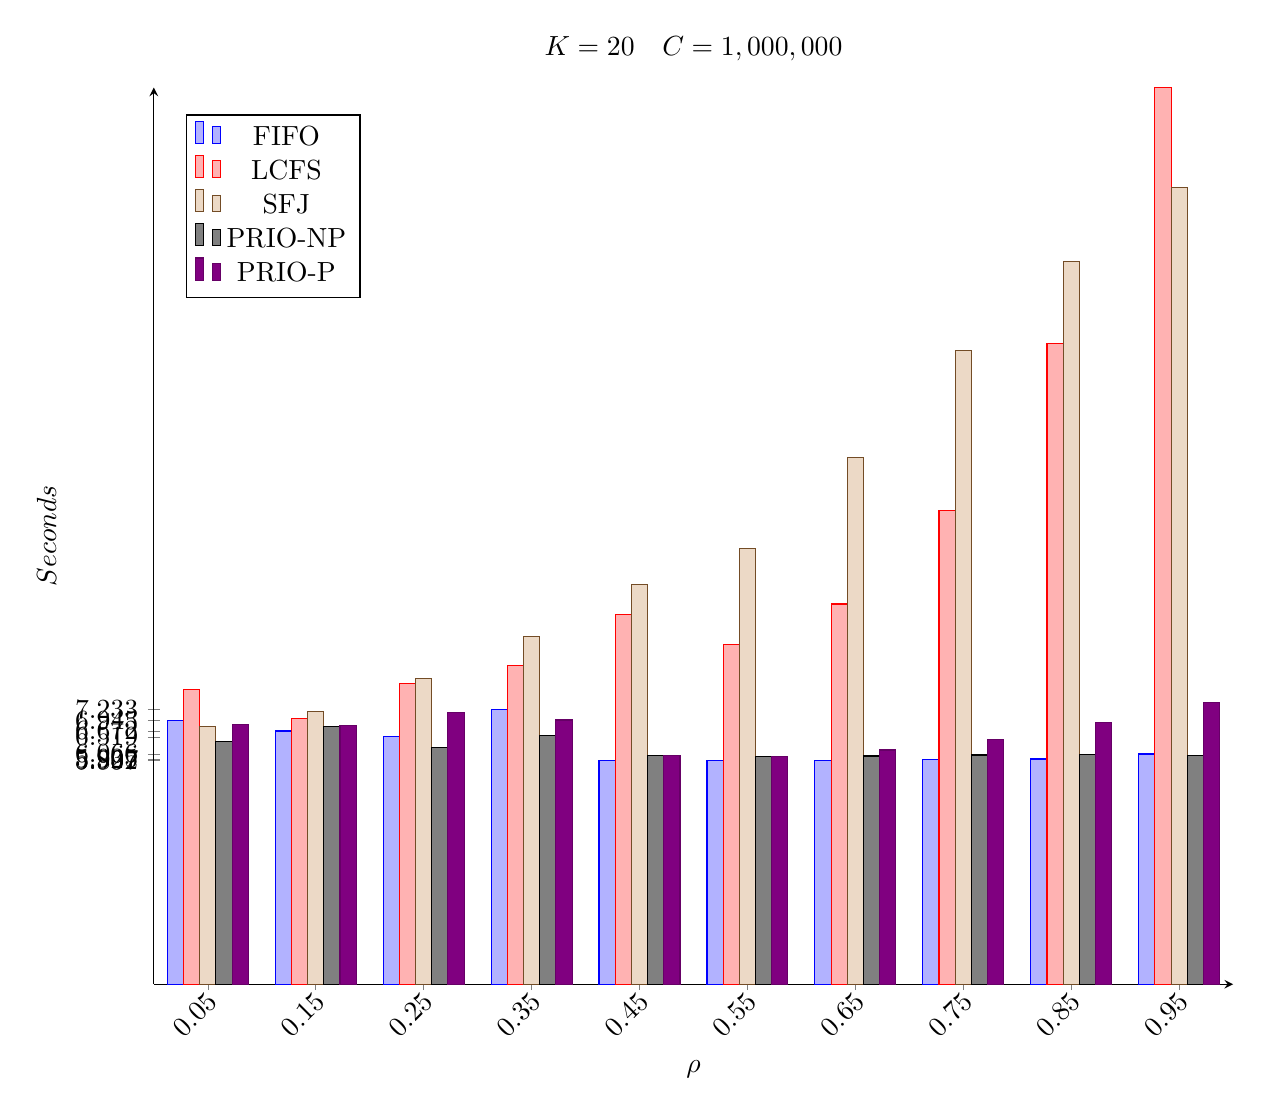
\begin{tikzpicture}[scale=1.0]
\begin{axis}[
    legend pos=north west,
    title= {$K=20 \quad C=1,000,000$},  
	ymin=0,
	y post scale=2,
	x post scale=2,
	ybar=0pt,
	bar width=0.015,
	enlargelimits={abs=0.5},
    xmin=0,
    xmax=1,
	xlabel = {$\rho$},
    ylabel = {$Seconds$},
	xtick=data,
	ytick=data,
	ticklabel style={
        /pgf/number format/fixed,
        /pgf/number format/precision=5
	},
	x tick label style={rotate=45, anchor=east, align=center, xshift=.1cm,yshift=-0.1cm},
	axis lines=left
	]
\addplot+[error bars/.cd,
y dir=both,y explicit]
coordinates {
    (0.05,6.945)
    (0.15,6.672)
    (0.25,6.519)
    (0.35,7.233)
    (0.45,5.897)
    (0.55,5.897)
    (0.65,5.902)
    (0.75,5.927)
    (0.85,5.935)
    (0.95,6.066)
};
\addplot+[error bars/.cd,
y dir=both,y explicit]
coordinates {
    (0.05,7.776)
    (0.15,6.991)
    (0.25,7.928)
    (0.35,8.388)
    (0.45,9.754)
    (0.55,8.943)
    (0.65,10.020)
    (0.75,12.485)
    (0.85,16.877)
    (0.95,23.630)
};
\addplot+[error bars/.cd,
y dir=both,y explicit]
coordinates {
    (0.05,6.800)
    (0.15,7.183)
    (0.25,8.054)
    (0.35,9.167)
    (0.45,10.529)
    (0.55,11.475)
    (0.65,13.886)
    (0.75,16.691)
    (0.85,19.046)
    (0.95,20.992)
};
\addplot+[error bars/.cd,
y dir=both,y explicit]
coordinates {
    (0.05,6.396)
    (0.15,6.799)
    (0.25,6.228)
    (0.35,6.552)
    (0.45,6.032)
    (0.55,5.990)
    (0.65,6.015)
    (0.75,6.039)
    (0.85,6.065)
    (0.95,6.018)
};
\addplot+[error bars/.cd,
y dir=both,y explicit]
coordinates {
    (0.05,6.853)
    (0.15,6.829)
    (0.25,7.167)
    (0.35,6.962)
    (0.45,6.023)
    (0.55,6.002)
    (0.65,6.173)
    (0.75,6.459)
    (0.85,6.907)
    (0.95,7.430)
};
\legend{FIFO, LCFS, SFJ, PRIO-NP, PRIO-P}
\end{axis}
\end{tikzpicture}
\\
For a constant queue capacity and completion size, where the queue capacity is large relative to the average number of customers in the system, the CLR  increases quickly at higher values of $\rho$. The FIFO and LCFS scheduling policies yield exactly the same CLR, since residual customers currently in service (because non-preemptive) does not change with the two policies. SJF shows a higher overal CLR, since this policy trades shorter average wait times for longer  queues. The priority queues show higher CLR for the lower priority queues, since these will be serviced less often. The preemptive priority queue has a higher CLR for all queues compared to the non-preemptive implementation. This is because there is a higher queue length due to pre-empted customers.
\\
For running time, the SJF and LCFS policies show increasing times, due to the linear computation needed to manage nonpreemption with these implementations. The other implementations show stable (or even decreasing) times. The decreasing times has no explanation, but the stable times are expected for this type of event-based simulation.
}
\bigskip
\newpage




%%%%%%%%%%%%%%%%%%%%%%
%%%%%%%%%%%%%%%%%%%%%%
%%%%%%%%%%%%%%%%%%%%%%

\textbf{Task 3 (Web Server with I/O)}
Let $K_{CPU} = 50, K_{I/O} = 30, C = 100, 000$ (this is the number of
customers leaving the system, possibly after each has made several trips to the CPU). Plot the average customer waiting time (and corresponding confidence intervals) against the value of $\rho = \lambda/\mu_{CPU}$ , for $\rho = 0.05, · · · , 0.95$, in increments of 0.10. Plot five curves: the average waiting time over all four queues, the average for the CPU queue only, and the average for each of the I/O disk queues. Also, define the CLR at any of the queues as the ratio of the number of customers dropped as they try to enter the queue over the total number of customers who tried to enter the same queue. Note that the denominator in this ratio may be different for the different queues; also assume that if a customer is dropped at any queue, it is lost. Plot the CLR for each of the four queues and the overall CLR for the system (for the overall CLR, any customer dropped at any queue is counted as lost).
\\
\medskip\\\texttt{
\\
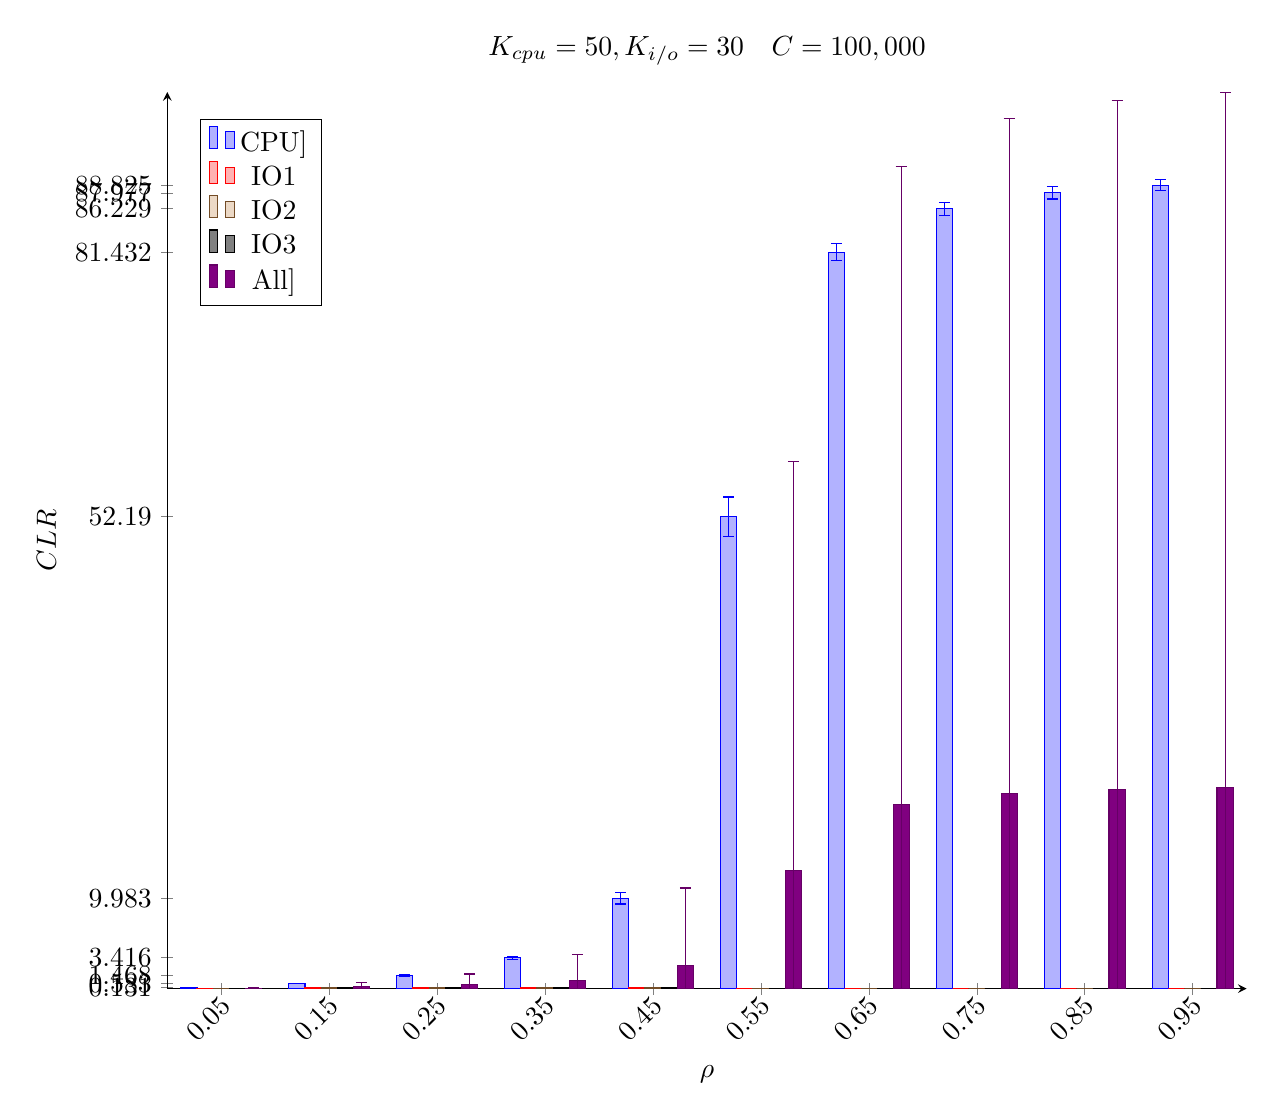
\begin{tikzpicture}
\begin{axis}[
    legend pos=north west,
    title= {$K_{cpu}=50, K_{i/o}=30 \quad C=100,000$},  
	ymin=0,
	y post scale=2,
	x post scale=2,
	ybar=0pt,
	bar width=0.015,
	enlargelimits={abs=0.5},
    xmin=0,
    xmax=1,
	xlabel = {$\rho$},
    ylabel = {$CLR$},
	xtick=data,
	ytick=data,
	ticklabel style={
        /pgf/number format/fixed,
        /pgf/number format/precision=5
	},
	x tick label style={rotate=45, anchor=east, align=center, xshift=.1cm,yshift=-0.1cm},
	axis lines=left
	]
\addplot+[error bars/.cd,
y dir=both,y explicit]
coordinates {
    (0.05,0.131) +- (0.0,0.009) 
    (0.15,0.583) +- (0.0,0.019) 
    (0.25,1.468) +- (0.0,0.063) 
    (0.35,3.416) +- (0.0,0.172) 
    (0.45,9.983) +- (0.0,0.625) 
    (0.55,52.190) +- (0.0,2.163) 
    (0.65,81.432) +- (0.0,0.940) 
    (0.75,86.229) +- (0.0,0.703) 
    (0.85,87.977) +- (0.0,0.667) 
    (0.95,88.825) +- (0.0,0.612) 
};
\addplot+[error bars/.cd,
y dir=both,y explicit]
coordinates {
    (0.05,0.028) +- (0.0,0.008) 
    (0.15,0.077) +- (0.0,0.015) 
    (0.25,0.115) +- (0.0,0.016) 
    (0.35,0.131) +- (0.0,0.017) 
    (0.45,0.103) +- (0.0,0.019) 
    (0.55,0.015) +- (0.0,0.010) 
    (0.65,0.000) +- (0.0,0.000)
    (0.75,0.000) +- (0.0,0.000)
    (0.85,0.000) +- (0.0,0.000)
    (0.95,0.000) +- (0.0,0.000)
};
\addplot+[error bars/.cd,
y dir=both,y explicit]
coordinates {
    (0.05,0.026) +- (0.0,0.009) 
    (0.15,0.078) +- (0.0,0.010) 
    (0.25,0.115) +- (0.0,0.015) 
    (0.35,0.130) +- (0.0,0.018) 
    (0.45,0.105) +- (0.0,0.017) 
    (0.55,0.014) +- (0.0,0.006) 
    (0.65,0.000) +- (0.0,0.001)
    (0.75,0.000) +- (0.0,0.000)
    (0.85,0.000) +- (0.0,0.000)
    (0.95,0.000) +- (0.0,0.000)
};
\addplot+[error bars/.cd,
y dir=both,y explicit]
coordinates {
    (0.05,0.028) +- (0.0,0.007) 
    (0.15,0.078) +- (0.0,0.014) 
    (0.25,0.115) +- (0.0,0.018) 
    (0.35,0.131) +- (0.0,0.015) 
    (0.45,0.104) +- (0.0,0.021) 
    (0.55,0.015) +- (0.0,0.007) 
    (0.65,0.000) +- (0.0,0.001) 
    (0.75,0.000) +- (0.0,0.000)
    (0.85,0.000) +- (0.0,0.000)
    (0.95,0.000) +- (0.0,0.000)
};
\addplot+[error bars/.cd,
y dir=both,y explicit]
coordinates {
    (0.05,0.053) +- (0.0,0.090)
    (0.15,0.204) +- (0.0,0.438)
    (0.25,0.453) +- (0.0,1.172)
    (0.35,0.952) +- (0.0,2.846)
    (0.45,2.574) +- (0.0,8.561)
    (0.55,13.059) +- (0.0,45.198)
    (0.65,20.358) +- (0.0,70.524)
    (0.75,21.557) +- (0.0,74.677)
    (0.85,21.994) +- (0.0,76.191)
    (0.95,22.206) +- (0.0,76.925)
};
\legend{CPU], IO1, IO2, IO3, All]}
\end{axis}
\end{tikzpicture}
\\
At low values of $\rho$, the CLR for the CPU and IO queues remains low but >0. As $\rho$ increases, the CPU queue becomes saturated and its CLR rises, resulting in a drop in CLR to the IO queues, since fewer (and then zero) jobs will be passed on these queues.
}
\bigskip
\newpage




%%%%%%%%%%%%%%%%%%%%%%
%%%%%%%%%%%%%%%%%%%%%%
%%%%%%%%%%%%%%%%%%%%%%

\textbf{Task 4 (Web Server with I/O)}
Let $K_{CPU} = 40, C = 100, 000$, and vary $\rho$ from 0.10 to 0.60 in
increments of 0.10. For each value of $\rho$, determine the minimum value $K_{I/O}$ of the I/O queues so that the CLR for any of these queues is less than 0.01 percent.
\\
\medskip\\\texttt{
\\
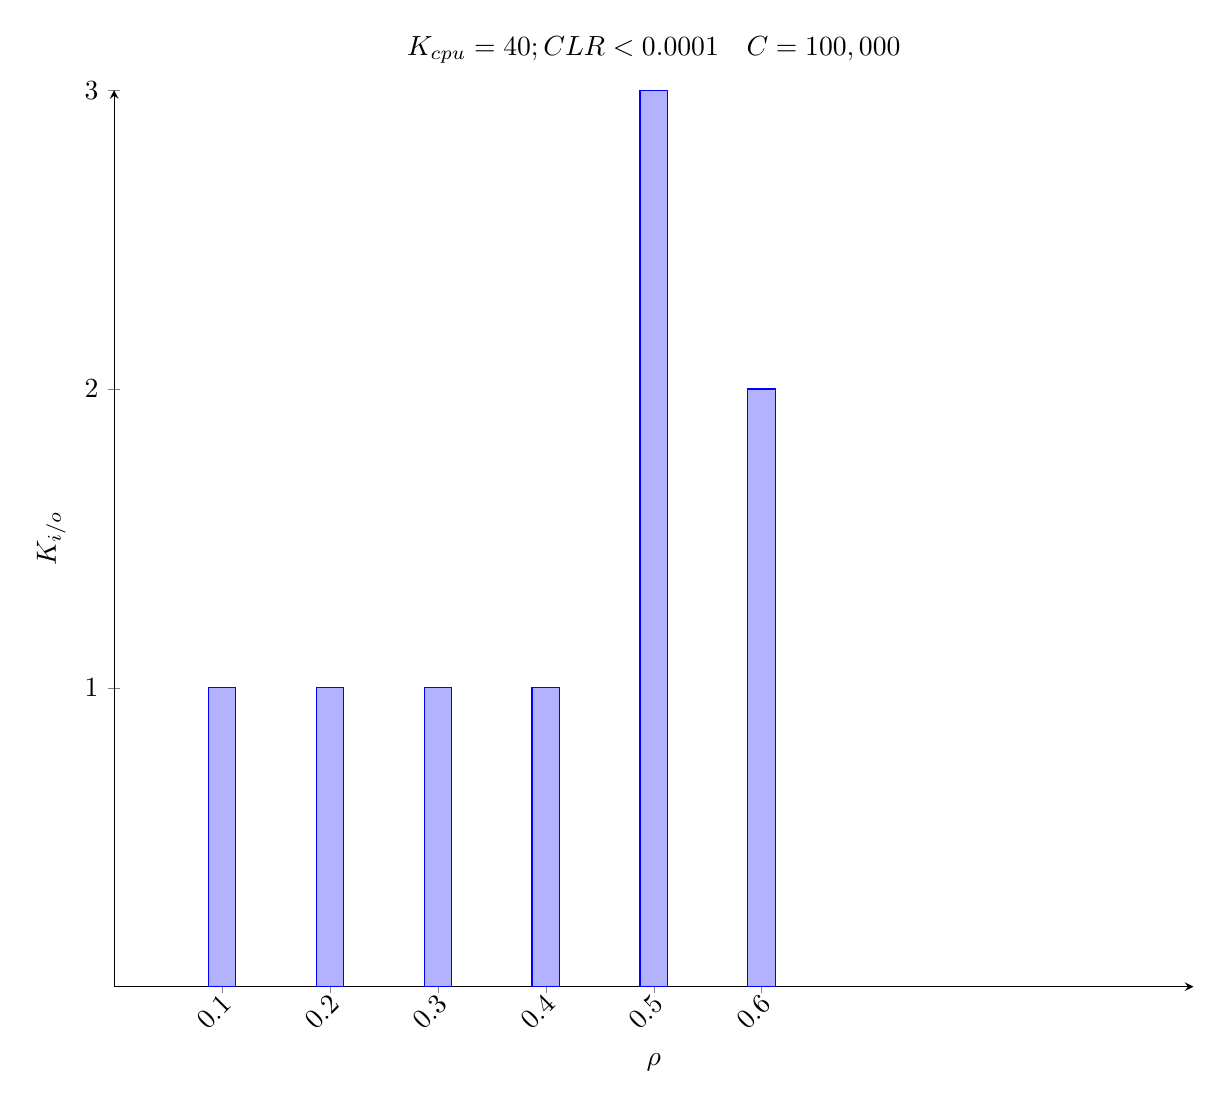
\begin{tikzpicture}
\begin{axis}[
    legend pos=north west,
    title= {$K_{cpu}=40; CLR<0.0001 \quad C=100,000$},  
	ymin=0,
	y post scale=2,
	x post scale=2,
	ybar=0pt,
	%bar width=0.015,
	enlargelimits={abs=0.5},
    xmin=0,
    xmax=1,
	xlabel = {$\rho$},
    ylabel = {$K_{i/o}$},
	xtick=data,
	ytick=data,
	ticklabel style={
        /pgf/number format/fixed,
        /pgf/number format/precision=5
	},
	x tick label style={rotate=45, anchor=east, align=center, xshift=.1cm,yshift=-0.1cm},
	axis lines=left
	]
\addplot+[error bars/.cd,
y dir=both,y explicit]
coordinates {
(0.10, 1)
(0.20, 1)
(0.30, 1)
(0.40, 1)
(0.50, 3)
(0.60, 2)
};
\end{axis}
\end{tikzpicture}
\\
At higher values of $\rho$ for a given $K_{CPU}$, a higher $K_{IO}$ is needed to maintain a low CLR, but at higher values of rho, the size of the IO queues is irrelevant.
}
\bigskip
\newpage



%%%%%%%%%%%%%%%%%%%%%%
%%%%%%%%%%%%%%%%%%%%%%
%%%%%%%%%%%%%%%%%%%%%%

\textbf{Task 5 (Web Server with I/O)}
Estimate the average number of times that a customer visits the CPU queue and each of the I/O disk queues. Plot these values against the value of $\rho$. Do they change as $\rho$ increases? Why or why not?
\\
\medskip\\\texttt{
\\
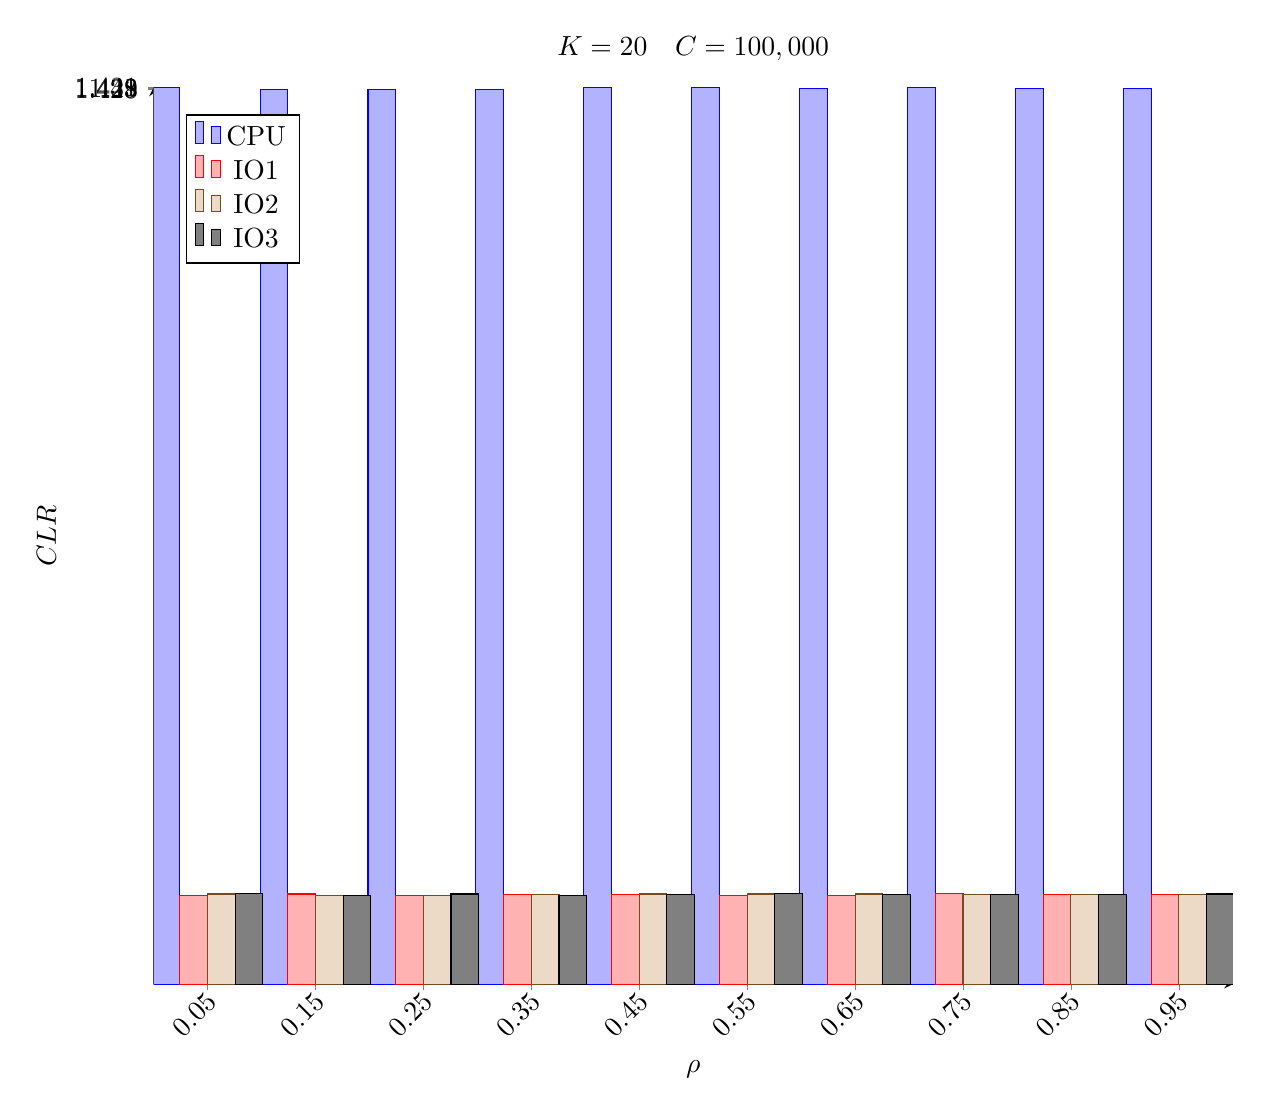
\begin{tikzpicture}[scale=1.0]
\begin{axis}[
    legend pos=north west,
    title= {$K=20 \quad C=100,000$},  
	ymin=0,
	y post scale=2,
	x post scale=2,
	ybar=0pt,
	enlargelimits={abs=0.5},
    xmin=0,
    xmax=1,
	xlabel = {$\rho$},
    ylabel = {$CLR$},
	xtick=data,
	ytick=data,
	ticklabel style={
        /pgf/number format/fixed,
        /pgf/number format/precision=5
	},
	x tick label style={rotate=45, anchor=east, align=center, xshift=.1cm,yshift=-0.1cm},
	axis lines=left
	]
\addplot+[error bars/.cd,
y dir=both,y explicit]
coordinates {
    (0.05, 1.431)
    (0.15, 1.428)
    (0.25, 1.428)
    (0.35, 1.428)
    (0.45, 1.431)
    (0.55, 1.431)
    (0.65, 1.429)
    (0.75, 1.431)
    (0.85, 1.430)
    (0.95, 1.430)
};
\addplot+[error bars/.cd,
y dir=both,y explicit]
coordinates {
    (0.05, 0.142)
    (0.15, 0.144)
    (0.25, 0.142)
    (0.35, 0.143)
    (0.45, 0.143)
    (0.55, 0.142)
    (0.65, 0.142)
    (0.75, 0.145)
    (0.85, 0.143)
    (0.95, 0.143)
};
\addplot+[error bars/.cd,
y dir=both,y explicit]
coordinates {
    (0.05, 0.144)
    (0.15, 0.142)
    (0.25, 0.142)
    (0.35, 0.143)
    (0.45, 0.144)
    (0.55, 0.144)
    (0.65, 0.144)
    (0.75, 0.143)
    (0.85, 0.143)
    (0.95, 0.143)
};
\addplot+[error bars/.cd,
y dir=both,y explicit]
coordinates {
    (0.05, 0.145)
    (0.15, 0.142)
    (0.25, 0.144)
    (0.35, 0.142)
    (0.45, 0.143)
    (0.55, 0.145)
    (0.65, 0.143)
    (0.75, 0.143)
    (0.85, 0.143)
    (0.95, 0.144)
};
\legend{CPU, IO1, IO2, IO3}
\end{axis}
\end{tikzpicture}
\\
A customer that exits the system will have visited the CPU and 0 or more IO queues based only the transition probabilities, not on the rate of customers entering the system.
}
\bigskip
\newpage

\bigskip


\label{last}
\end{document}

